% Porter model
% Author: Charles-Axel Dein
\documentclass[preview]{standalone} 

\usepackage[hmargin=2cm,vmargin=1cm]{geometry}
\renewcommand{\rmdefault}{bch} % change default font

\usepackage[english]{babel}
\usepackage[normalem]{ulem}
\usepackage[utf8]{inputenc}
\usepackage{tikz} 
\usetikzlibrary{arrows,decorations.pathmorphing,backgrounds,fit,positioning,shapes.symbols,chains}
%%%%%%%%%%%%%%%%%%%%%%%%%%%%%%%%%%%%
%%% BEGIN DOCUMENT
\begin{document}

\begin{figure}[h]

\centering
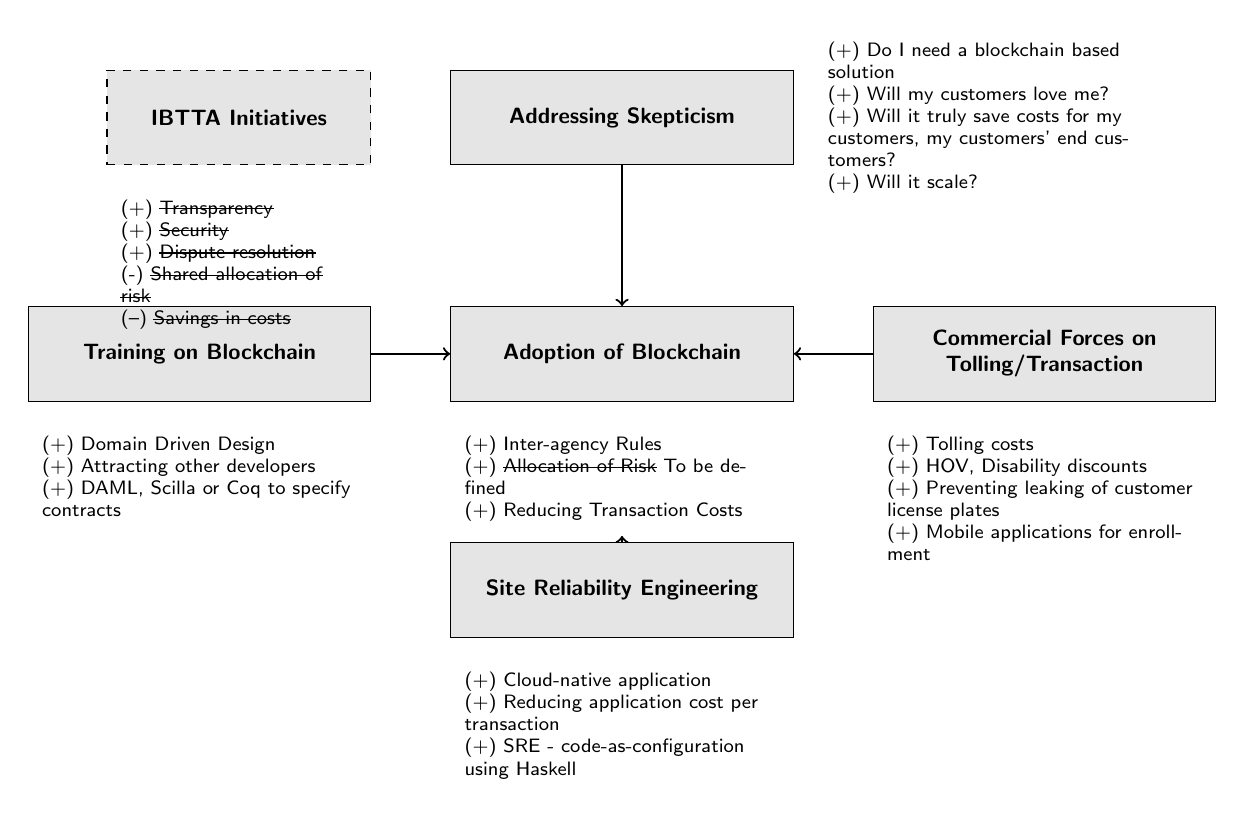
\begin{tikzpicture}
[node distance = 1cm, auto,font=\footnotesize,
% STYLES
every node/.style={node distance=3cm},
% The comment style is used to describe the characteristics of each force
comment/.style={rectangle, inner sep= 5pt, text width=4cm, node distance=0.25cm, font=\scriptsize\sffamily},
% The force style is used to draw the forces' name
force/.style={rectangle, draw, fill=black!10, inner sep=5pt, text width=4cm, text badly centered, minimum height=1.2cm, font=\bfseries\footnotesize\sffamily}] 

% Draw forces
\node [force] (adoptionOfBlockchain) {Adoption of Blockchain};
\node [force, above of=adoptionOfBlockchain] (mentoring) {Addressing Skepticism};
\node [force, text width=3cm, dashed, left=1cm of mentoring] (iag) {IBTTA Initiatives};
\node [force, left=1cm of adoptionOfBlockchain] (training) {Training on Blockchain};
\node [force, right=1cm of adoptionOfBlockchain] (vendors) {Commercial Forces on Tolling/Transaction};
\node [force, below of=adoptionOfBlockchain] (sre) {Site Reliability Engineering};

%%%%%%%%%%%%%%%
% Change data from here

% RIVALRY
\node [comment, below=0.25 of adoptionOfBlockchain] (comment-adoptionOfBlockchain) {(+) Inter-agency Rules\\
(+) \sout{Allocation of Risk} To be defined\\
(+) Reducing Transaction Costs};

% SUPPLIERS
\node [comment, below=0.25cm of training] {(+) Domain Driven Design\\
(+) Attracting other developers\\
(+) DAML, Scilla or Coq to specify contracts};

% SUBSTITUTES
\node [comment, right=0.25 of mentoring] {(+) Do I need a blockchain based solution\\
  (+) Will my customers love me?\\
  (+) Will it truly save costs for my customers, my customers' end customers?\\
  (+) Will it scale?
};

% USERS
\node [comment, below=0.25 of vendors] {(+) Tolling costs\\
  (+) HOV, Disability discounts \\
  (+) Preventing leaking of customer license plates \\
  (+) Mobile applications for enrollment
  };

% NEW ENTRANTS
\node [comment, below=0.25 of sre] {(+) Cloud-native application \\
  (+) Reducing application cost per transaction \\
  (+) SRE - code-as-configuration using Haskell
};

% PUBLIC POLICIES
\node [comment, text width=3cm, below=0.25 of iag] {(+) \sout{Transparency}\\
(+) \sout{Security} \\
(+) \sout{Dispute resolution} \\
(-) \sout {Shared allocation of risk}\\
(--) \sout{Savings in costs}};

%%%%%%%%%%%%%%%%

% Draw the links between forces
\path[->,thick] 
(mentoring) edge (adoptionOfBlockchain)
(training) edge (adoptionOfBlockchain)
(vendors) edge (adoptionOfBlockchain)
(sre) edge (comment-adoptionOfBlockchain);

\end{tikzpicture} 
\caption{Adoption of Blockchain in Tolling and Transportation}
\label{fig:6forces}
\end{figure}

\end{document}